\documentclass[cn]{report}
\usepackage{minted}
\setminted{autogobble}
\usepackage{placeins}

\let\t\texttt
\setmonofont[Scale=0.85]{Cascadia Code PL}

\begin{document}
    \title{Yet Another Raytracer}
    \maketitle
    \tableofcontents
    \newpage

    \section{简介}
    本项目使用 C++ 实现了一个纯 CPU 的光线追踪器,包含了下述特性(后附相关的代码位置):

    \begin{enumerate}
        \item 算法选型:路径追踪(PT)、随机渐进光子映射(SPPM) \hfill\t{src/renders/*.cpp}
        \item 基于牛顿法的旋转 Bezier 曲面绘制 \hfill\t{src/objects/rotate\_bezier.cpp}
        \item 基于 AABB 和 BVH 的复杂三角网格求交加速 \hfill\t{src/objects/bvh.cpp, src/utils/aabb.cpp}
        \item 景深 \hfill\t{src/core/camera.cpp [PerspectiveCamera::generateRay()]}
        \item 软阴影 \hfill\t{src/core/light.cpp}
        \item 基于超采样和 tent filter 的抗锯齿 \hfill\t{src/renderers/*.cpp [Render()]}
        \item 纹理映射和贴图 \hfill \t{src/objects/*.cpp [SimpleObject3D::AmbientColorAtHit()]}
        \item 焦散\hfill \t{src/renderers/photon\_mapping.cpp}
    \end{enumerate}

    本项目代码以 GPL 3.0 协议开源,源代码仓库位于 \url{https://github.com/SharzyL/rt}。

    % \def\nogallery{}
    \section{结果}
    为了展示光线追踪器的特性,我们设计了若干个场景,使用 PT 或者 SPPM 渲染器渲染。渲染使用的参数见表~\ref{tab:render-args},渲染结果见后文附图。
    \begin{table}[htbp]
        \centering
        \small
        \begin{tabular}{lll}\toprule
            编号 & 图片内容 & 渲染参数 \\ \midrule
            \ref{fig:cornell-2ball} & 折射和反射(PT) & \t{./build/RT -i scenes/cornell-2ball.yml -p4 -s1024} \\
            \ref{fig:cornell-2ball-sppm} & 折射和反射(SPPM) & \t{./build/RT\_sppm -i scenes/cornell-2ball.yml -p 10000000 -n 50 -r 0.008} \\
            \ref{fig:bezier} & 贝塞尔旋转曲面 & \t{./build/RT -i scenes/cornell-bezier.yml -p4 -s512} \\
            \ref{fig:bleeding} & Color Bleeding & \t{./build/RT -i scenes/bleeding.yml -p4 -s512} \\
            \ref{fig:depth} & 景深 & \t{./build/RT -i scenes/cornell-depth.yml -p4 -s1024} \\
            \ref{fig:dragon} & 龙 & \t{./build/RT -i scenes/dragon.yml -p4 -s512} \\
            \ref{fig:m4a1} & M4A1 & \t{./build/RT -i scenes/m4a1.yml -p4 -s512} \\
            \ref{fig:caustics} & 焦散 & \t{./build/RT\_sppm -i scenes/caustics.yml -p 10000000 -n 50 -r 0.008} \\
            \bottomrule
        \end{tabular}
        \caption{}\label{tab:render-args}
    \end{table}

\ifdefined\nogallery\else
    \begin{figure}[htbp]
        \centering
        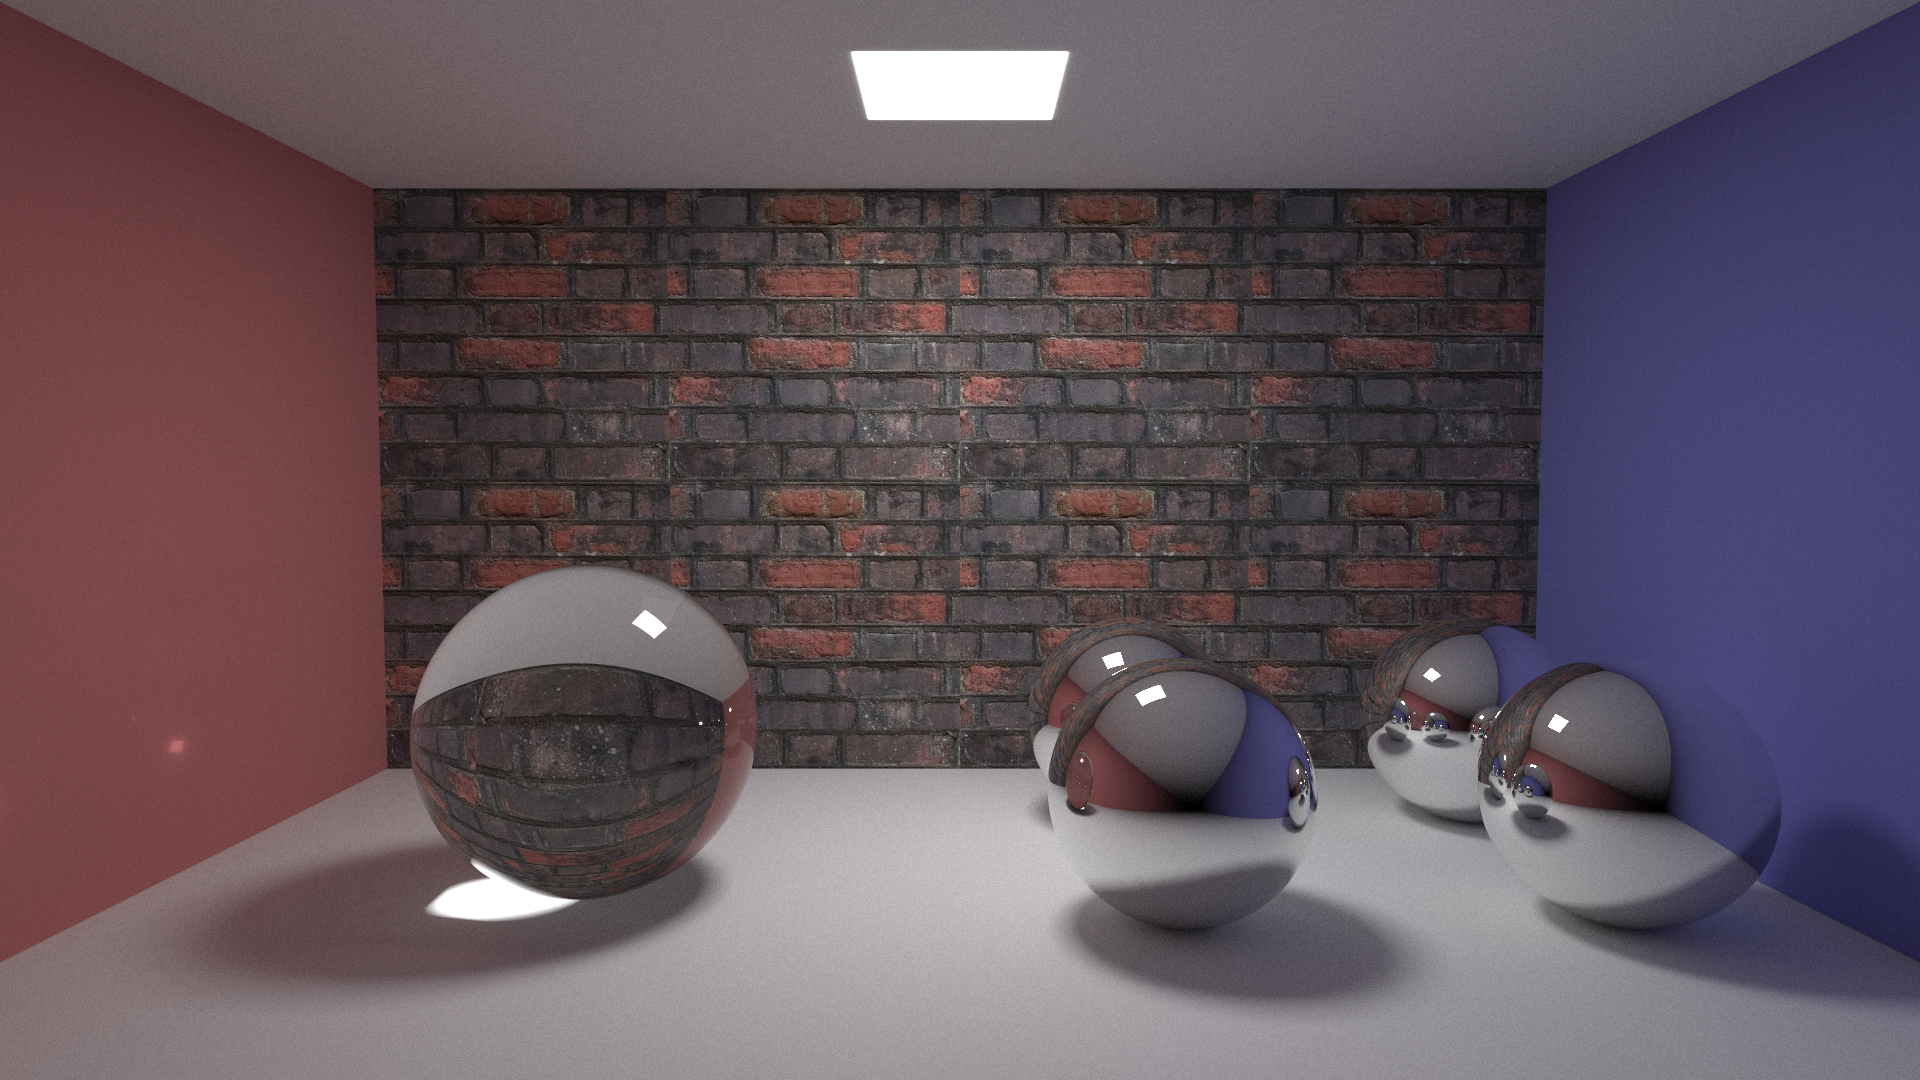
\includegraphics[width=\linewidth]{../results/cornell-2ball.png}
        \caption{折射和反射(PT)}
        \label{fig:cornell-2ball}
    \end{figure}

    \begin{figure}[htbp]
        \centering
        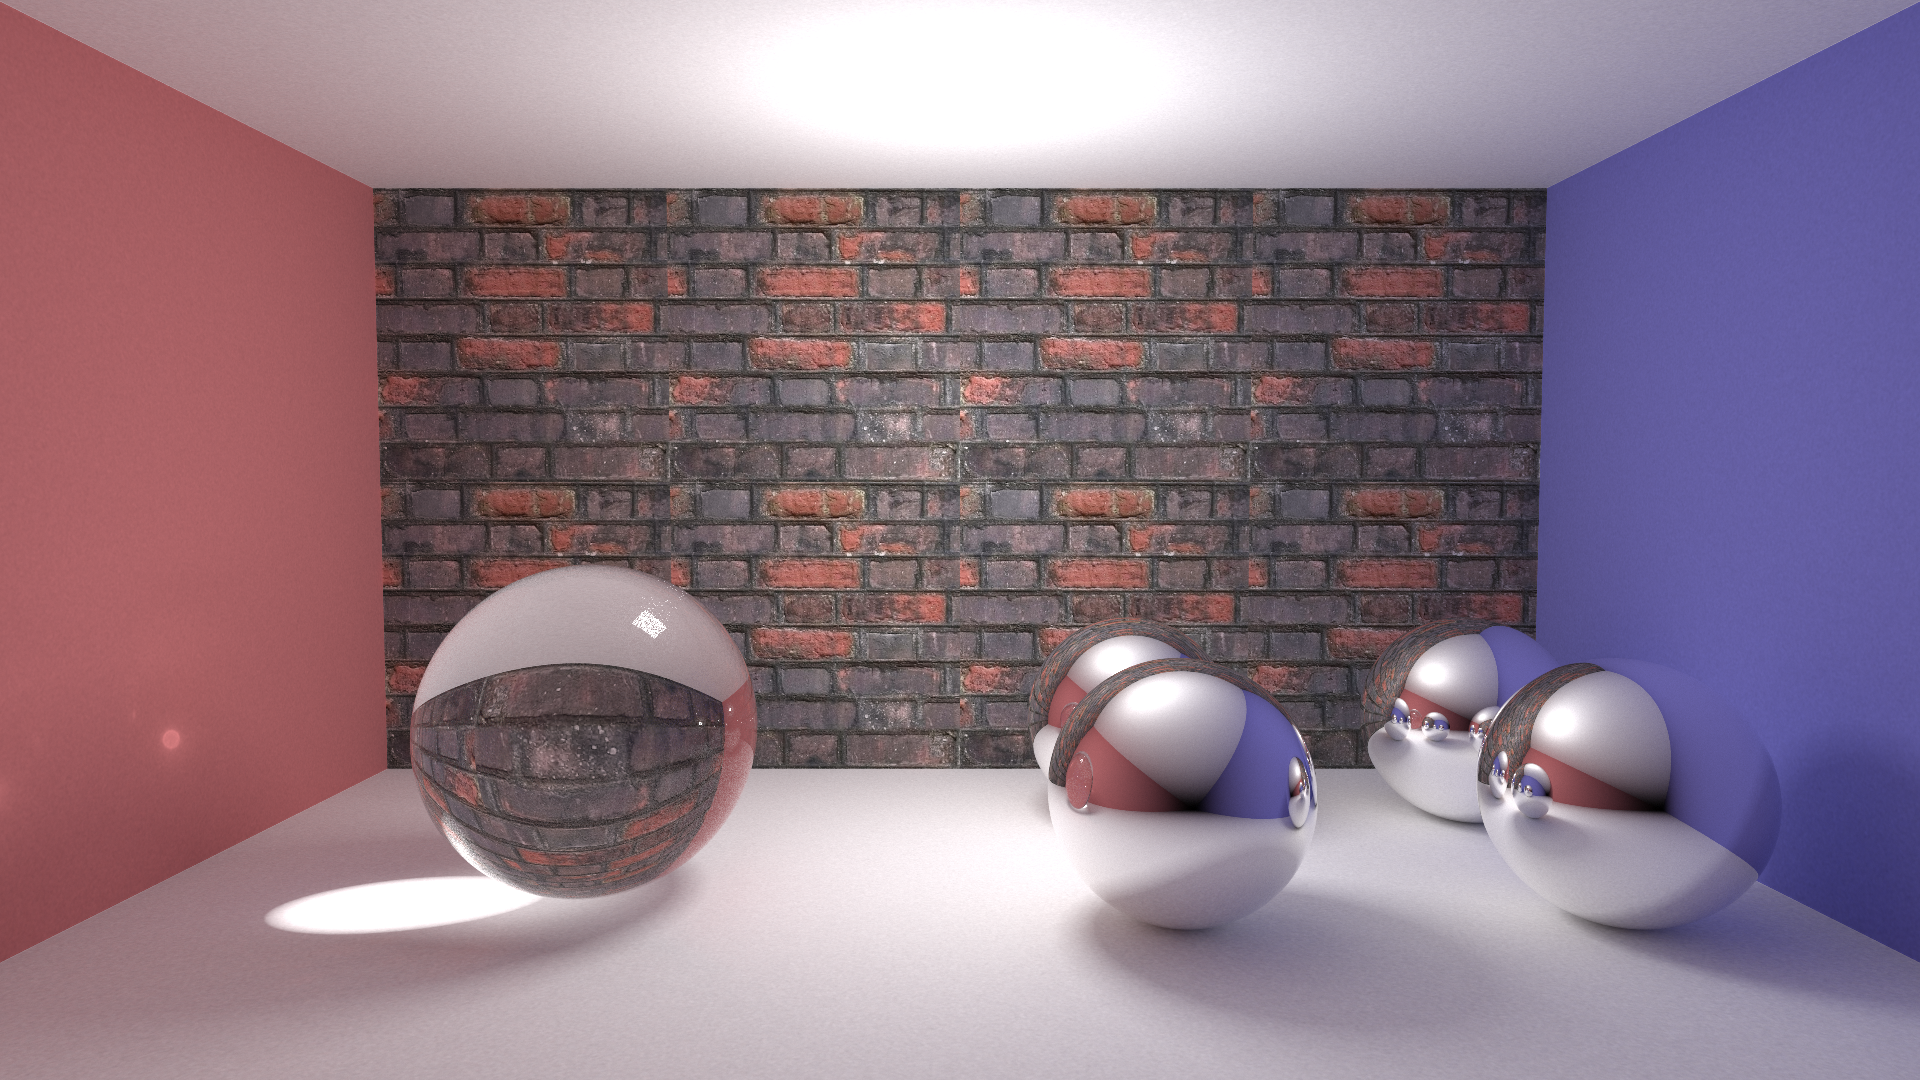
\includegraphics[width=\linewidth]{../results/cornell-2ball-sppm.png}
        \caption{折射和反射(SPPM)}
        \label{fig:cornell-2ball-sppm}
    \end{figure}

    \begin{figure}[htbp]
        \centering
        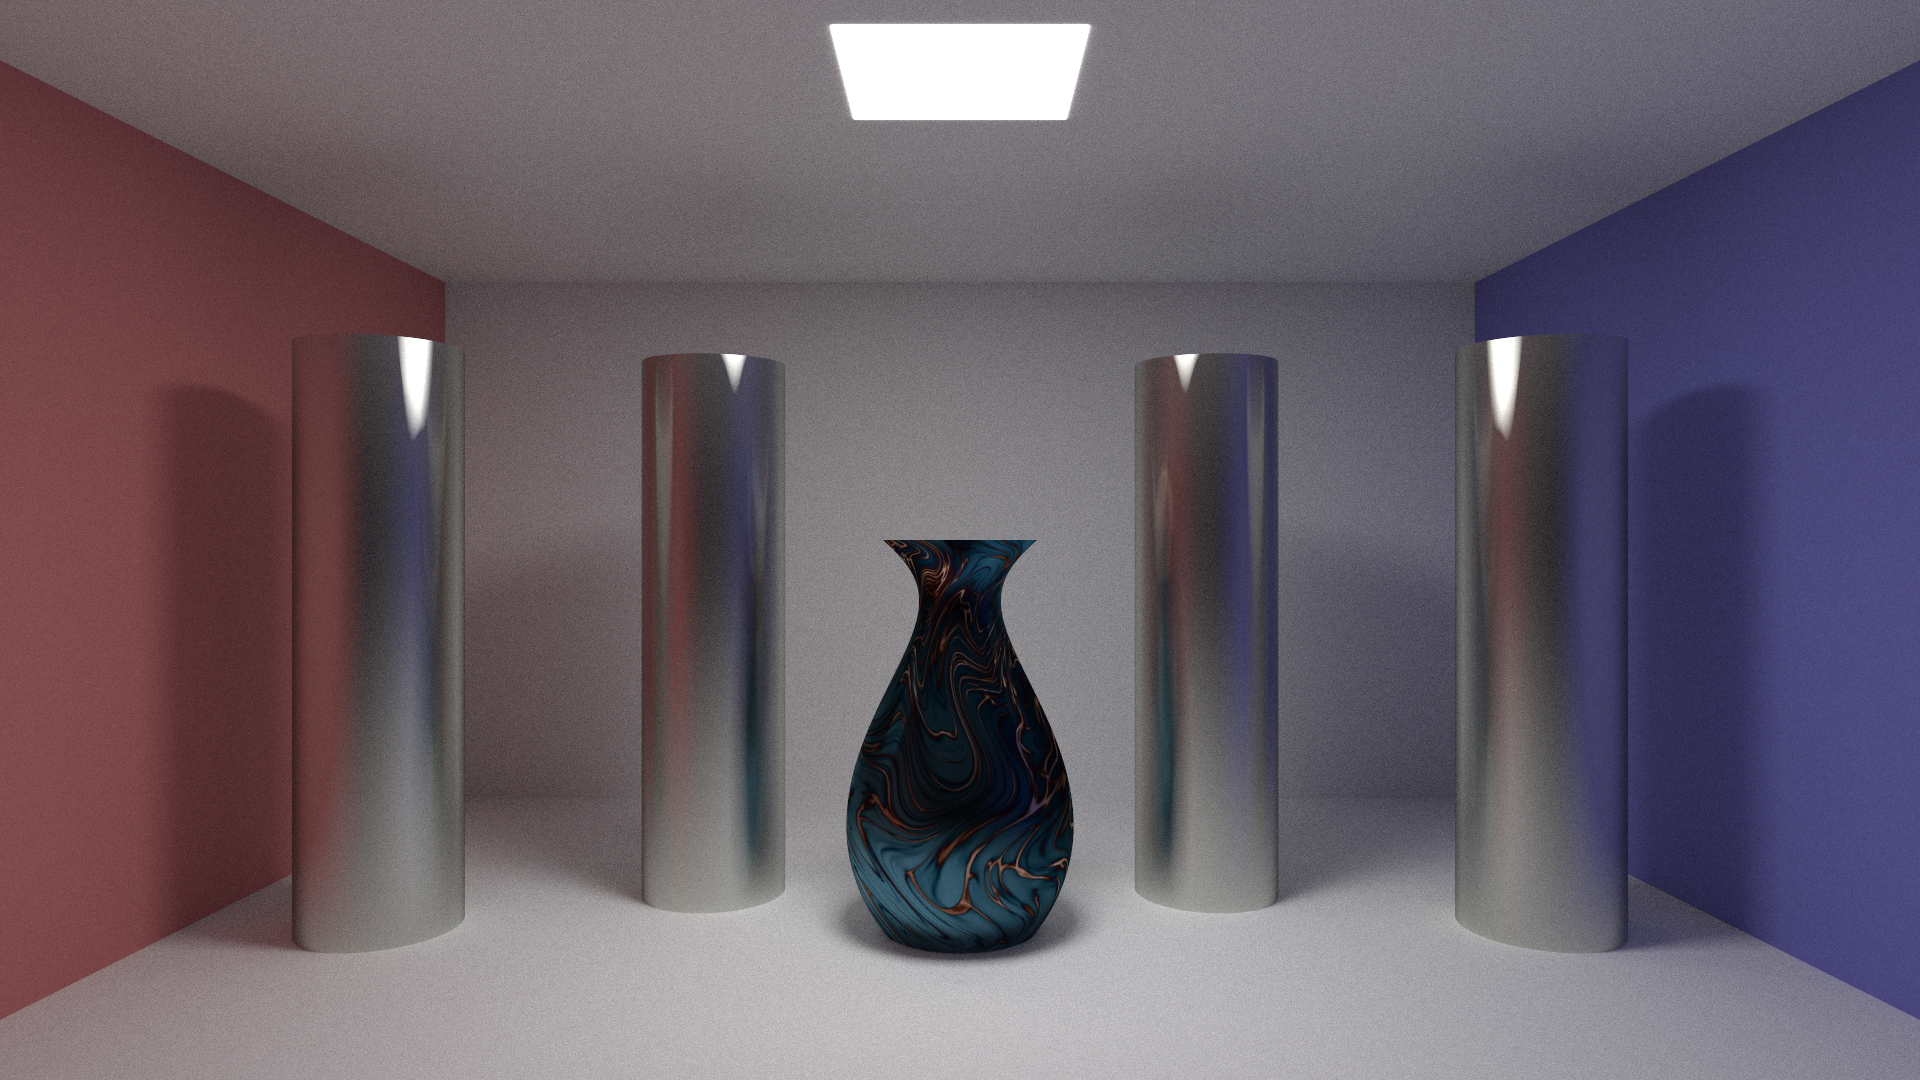
\includegraphics[width=\linewidth]{../results/cornell-bezier.png}
        \caption{贝塞尔旋转曲面}
        \label{fig:bezier}
    \end{figure}

    \begin{figure}[htbp]
        \centering
        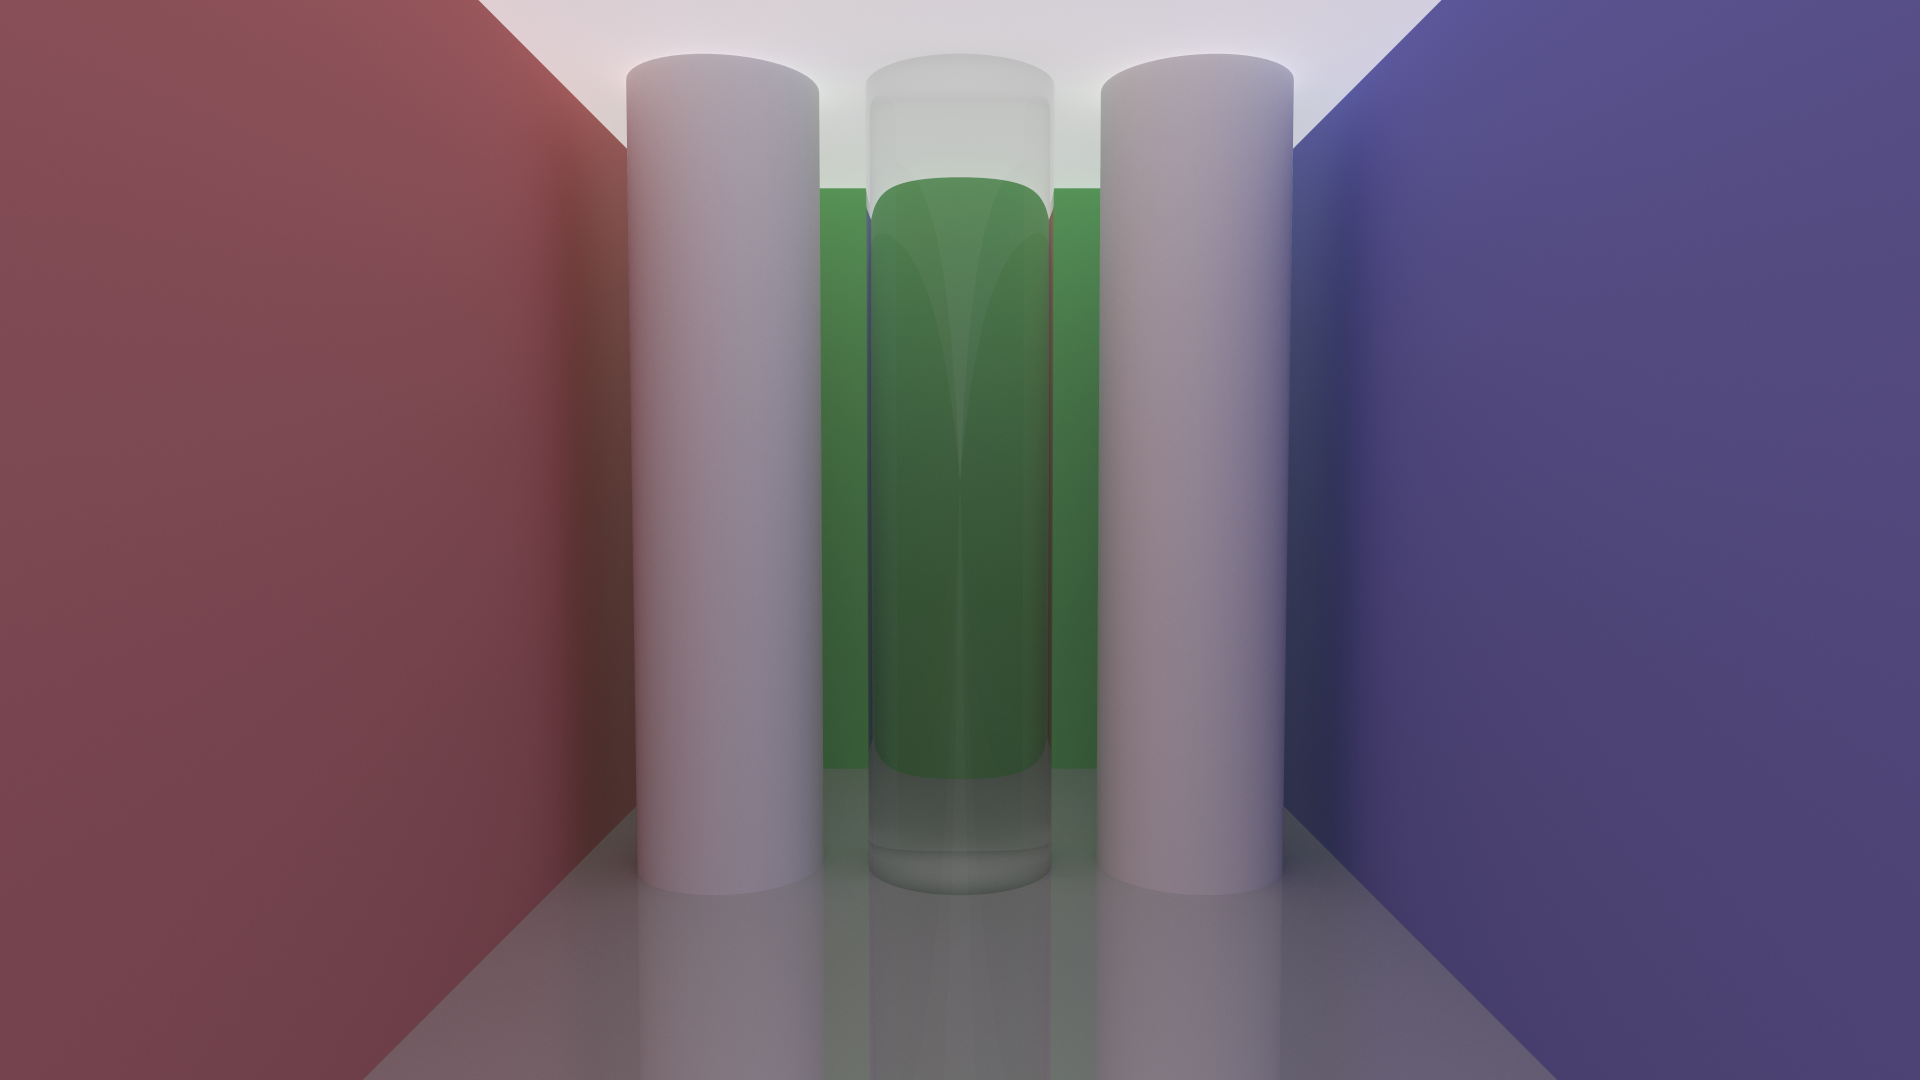
\includegraphics[width=\linewidth]{../results/bleeding.png}
        \caption{景深}
        \label{fig:bleeding}
    \end{figure}

    \begin{figure}[htbp]
        \centering
        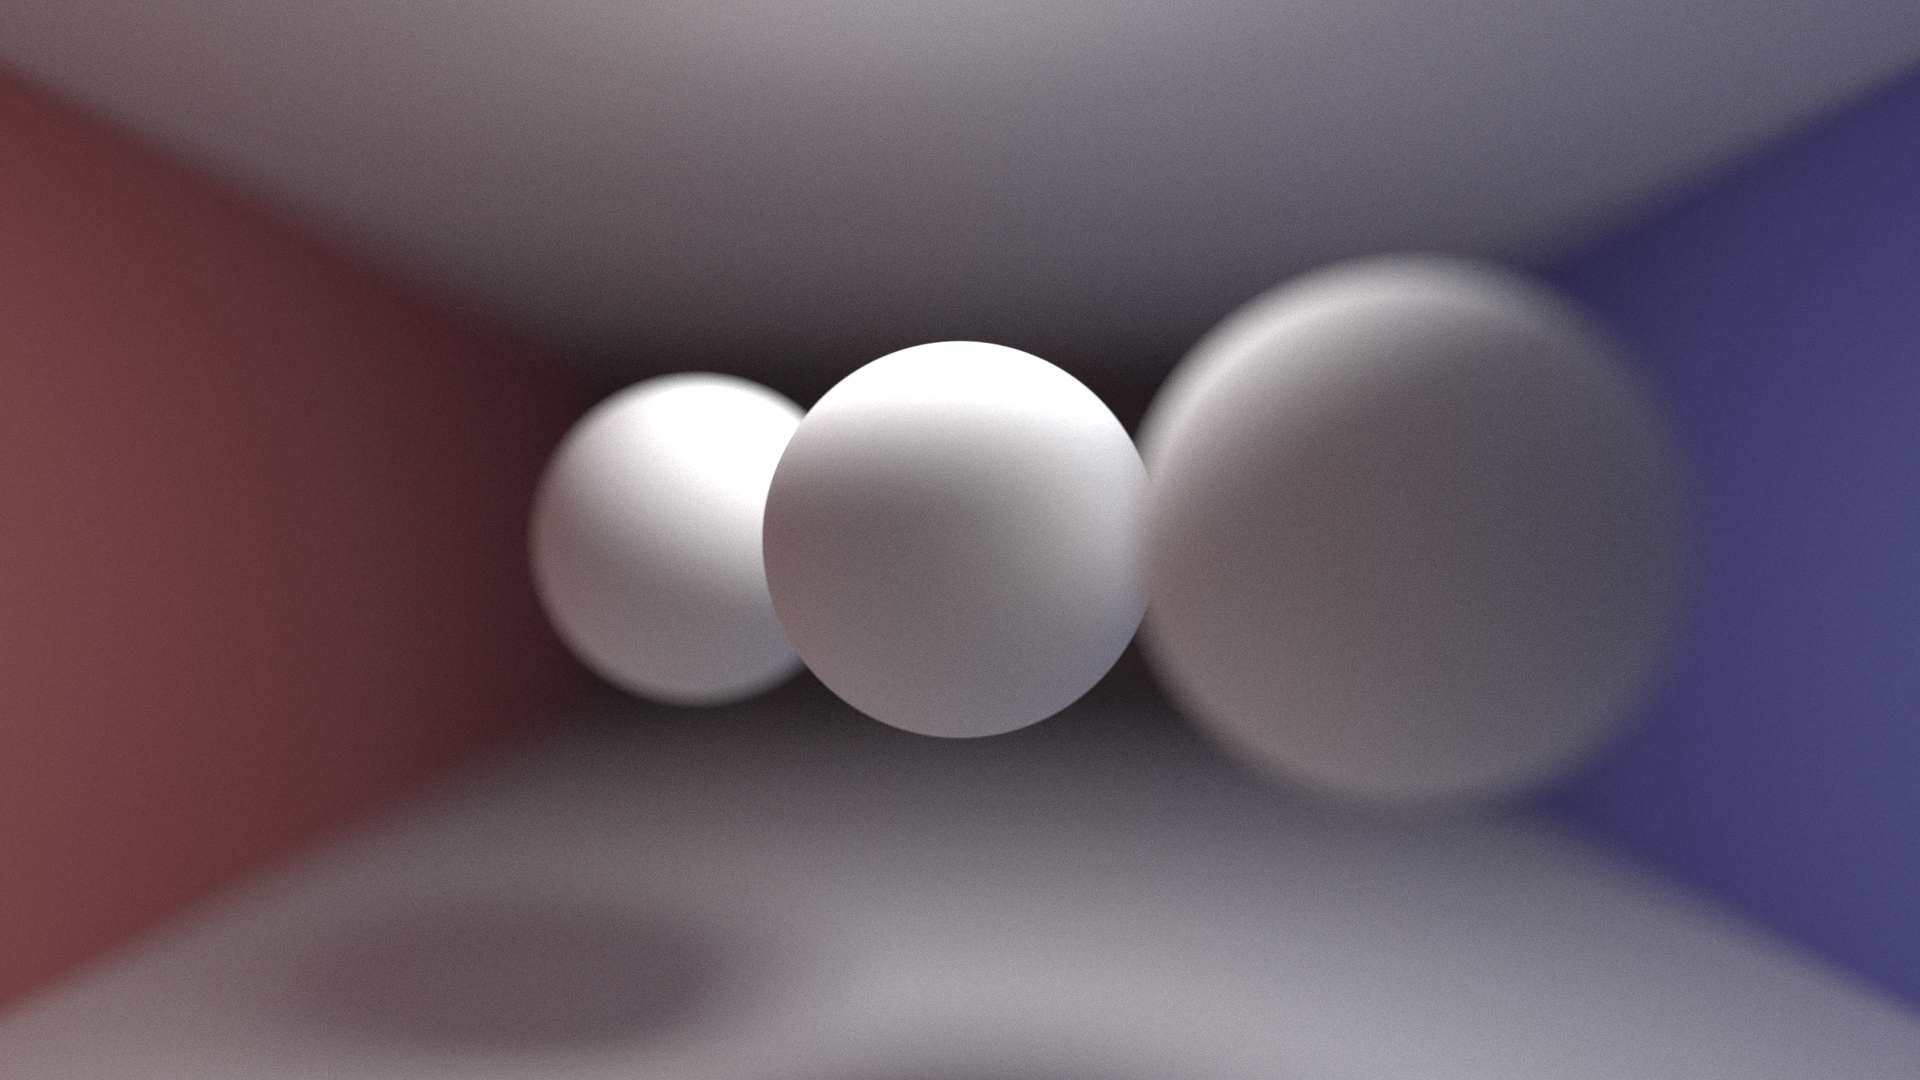
\includegraphics[width=\linewidth]{../results/cornell-depth.png}
        \caption{Color Bleeding}
        \label{fig:depth}
    \end{figure}

    \begin{figure}[htbp]
        \centering
        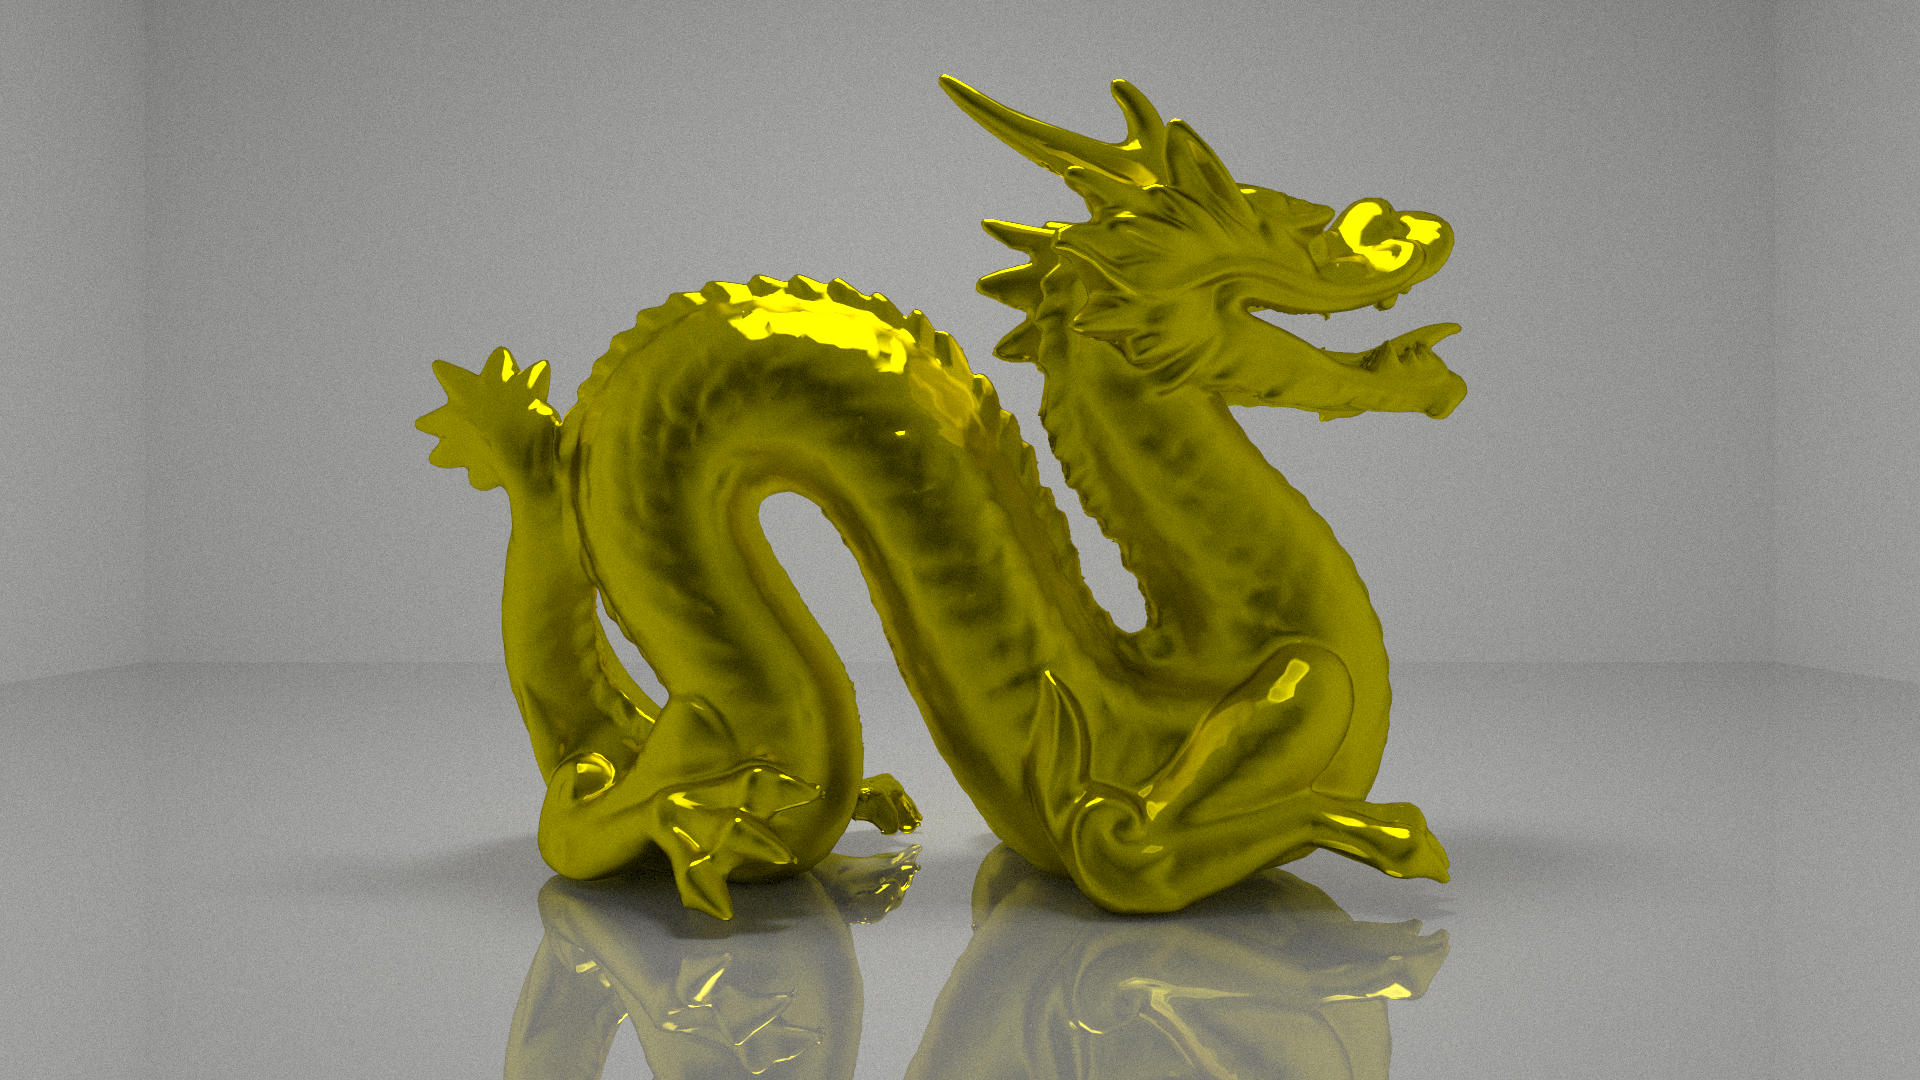
\includegraphics[width=\linewidth]{../results/dragon.png}
        \caption{龙}
        \label{fig:dragon}
    \end{figure}

    \begin{figure}[htbp]
        \centering
        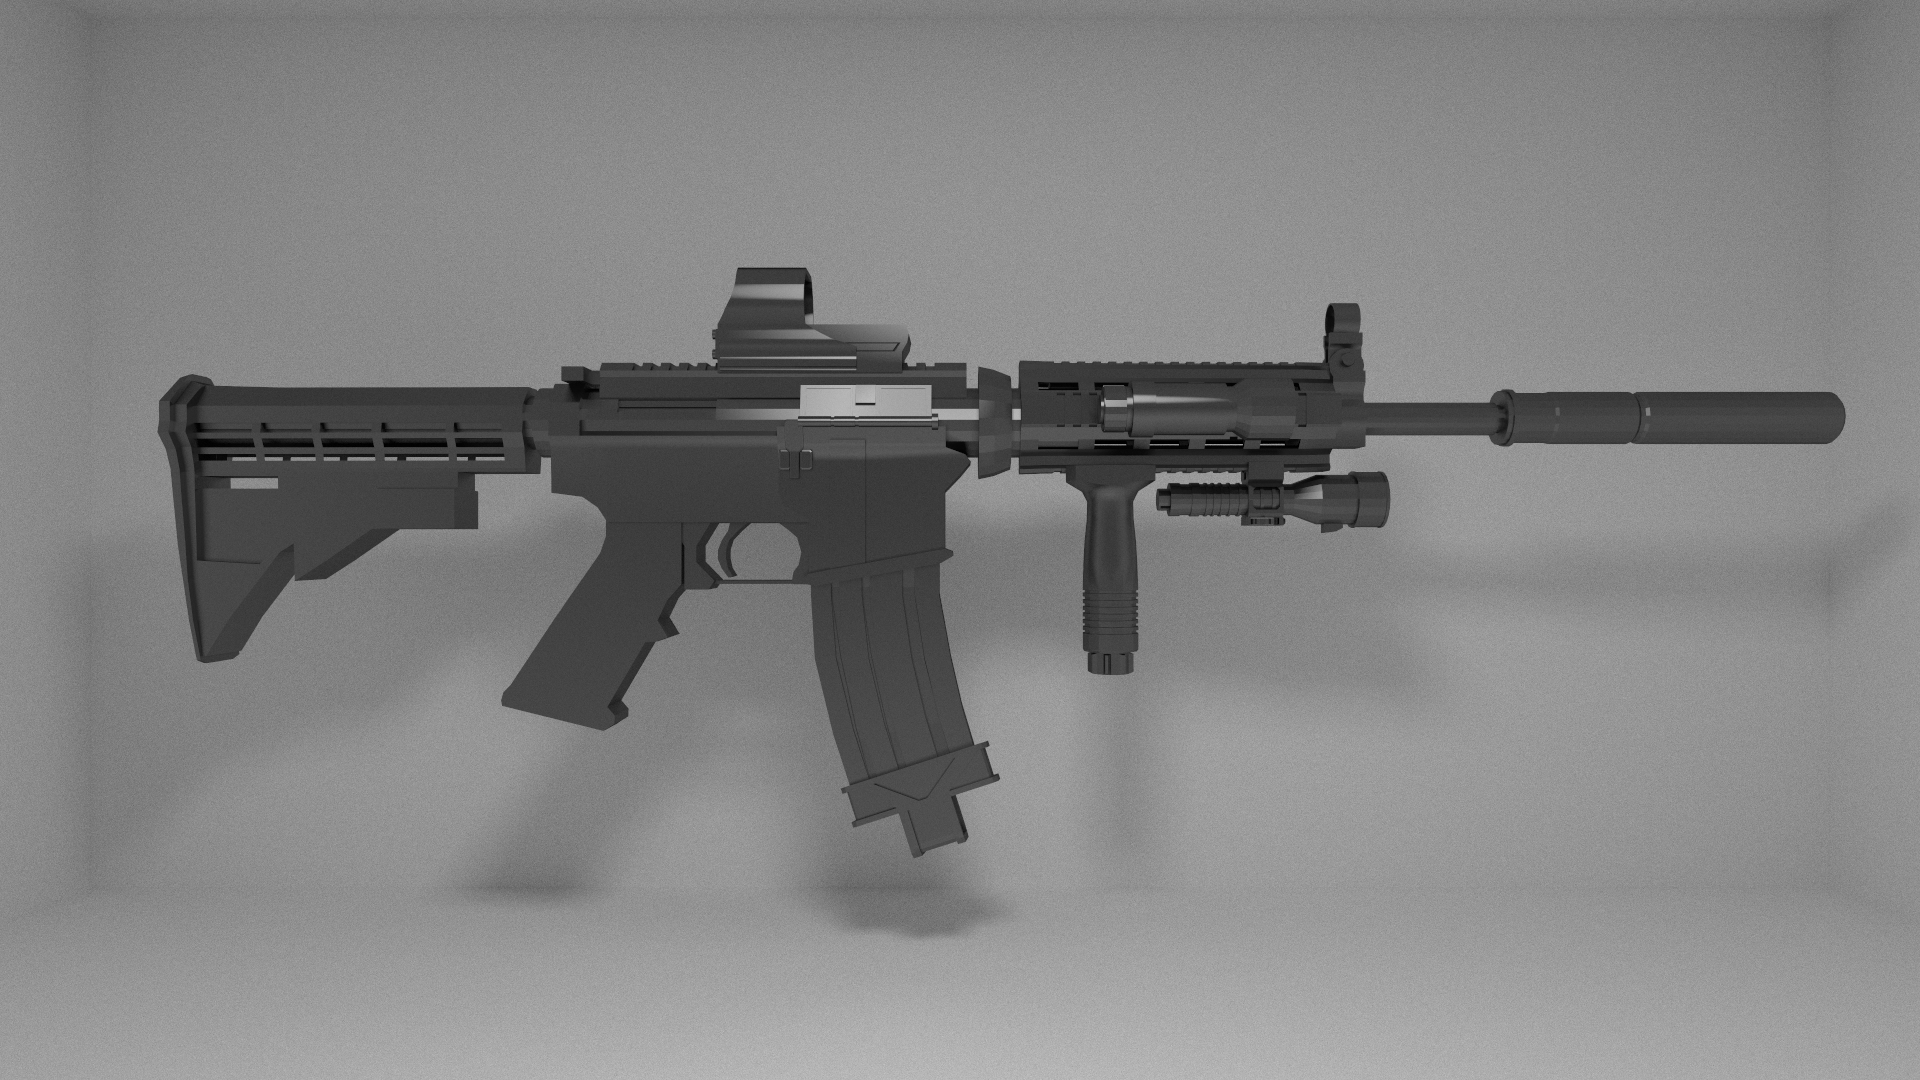
\includegraphics[width=\linewidth]{../results/m4a1.png}
        \caption{M4A1}
        \label{fig:m4a1}
    \end{figure}

    \begin{figure}[htbp]
        \centering
        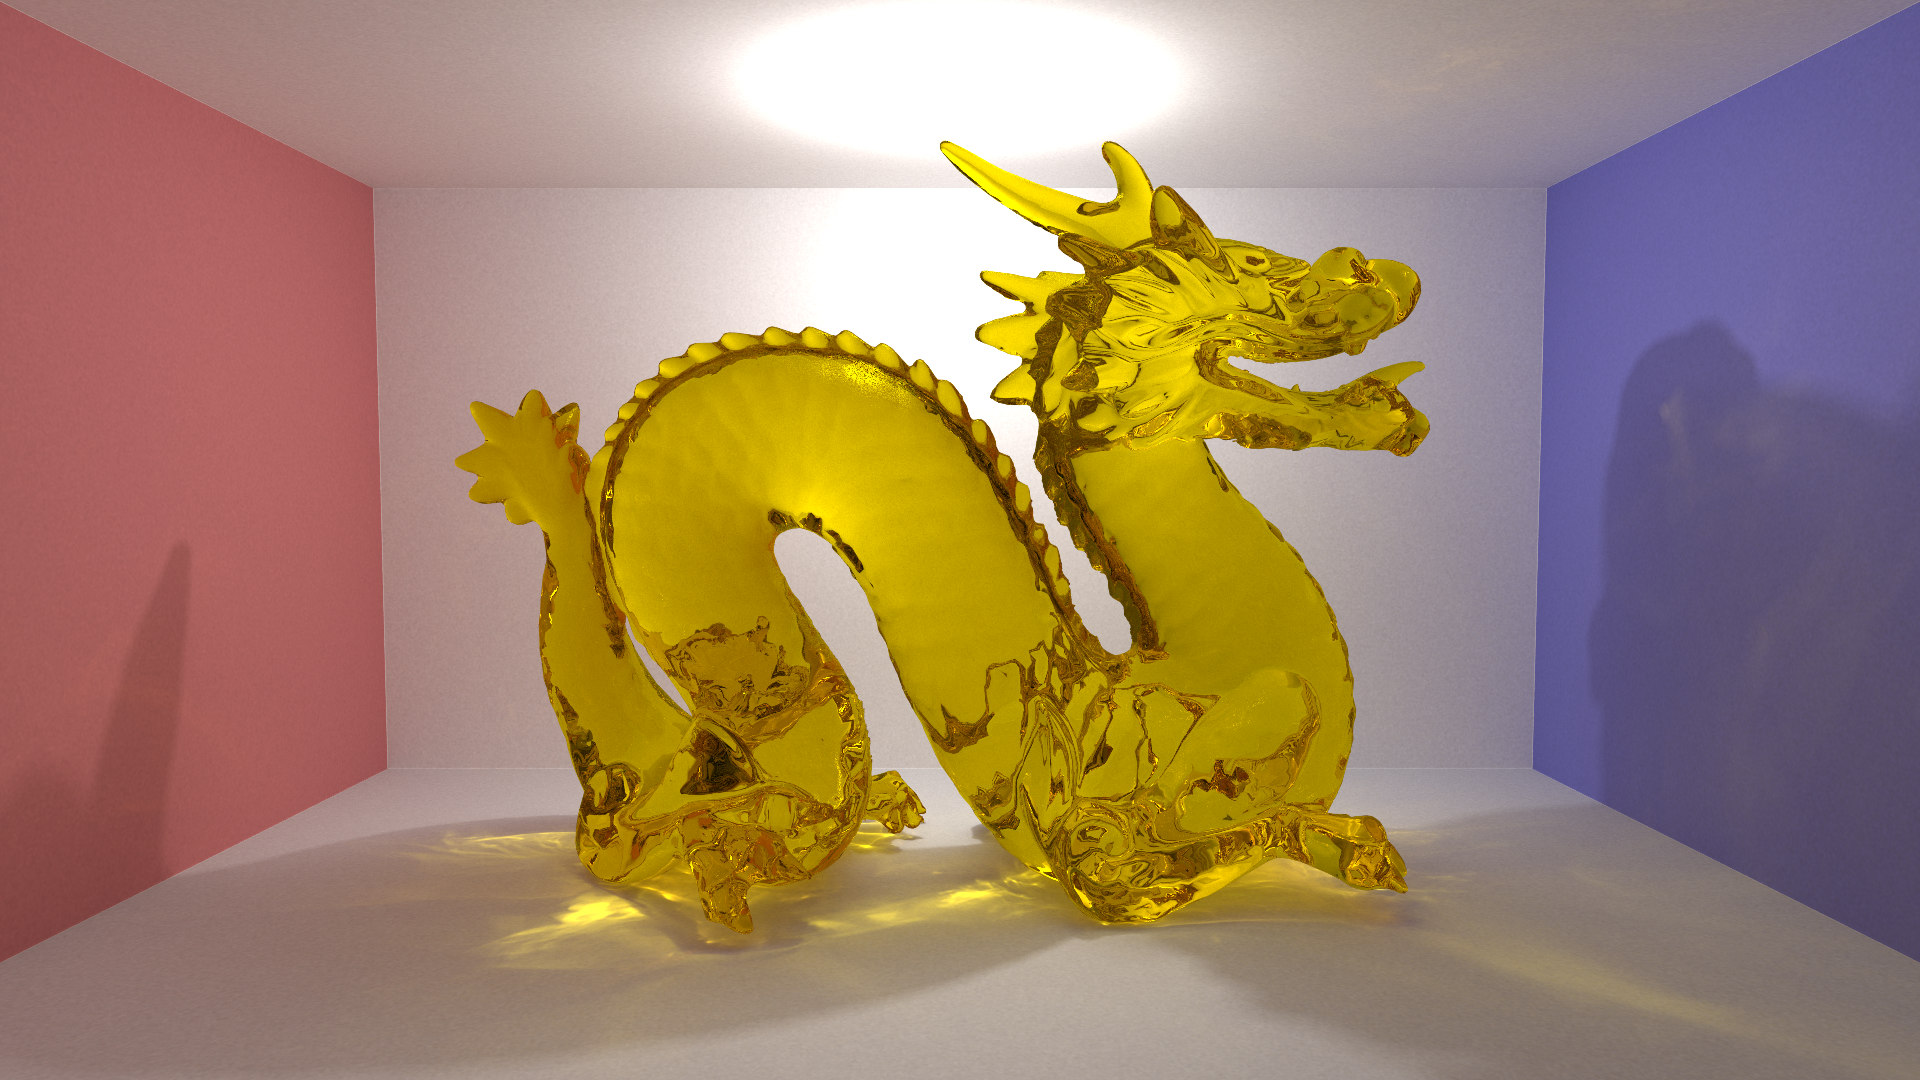
\includegraphics[width=\linewidth]{../results/caustics.png}
        \caption{焦散}
        \label{fig:caustics}
    \end{figure}
    \fi

    \FloatBarrier

    \section{实现细节}

    \subsection{路径追踪算法}
    为了求出某个像素的颜色,我们考察一条从镜头发出的光线,求出该光线和场景的第一个交点。我们通过 \t{Material} 和 \t{Hit} 类提供的相关方法计算出交点出的物体颜色,并且根据交点处材料的特性采样一条射出的光线,以及这条光线对应的 BRDF 函数值。对于射出的光线,递归地执行相同的步骤,直到追踪深度大于给定的阈值,从而得到采样光线的颜色 \t{sample\_ray\_color},最后通过 \begin{align}\t{emission\_color + ambient\_color * sample\_ray\_color * brdf} \end{align} 计算出光线的颜色。

    \subsection{SPPM 算法}

    首先我们考虑 PPM 算法。在 PPM 算法中,首先从相机出发,对于每个像素发射出一条光线,在场景内追踪这条光线,直到光线到达漫反射面或者到达场景之外为止。如果光线到达了漫反射面,则在光线和这个表面的交点处记录一个点(我们称之为可见点)。在可见点上记录光线到达这里的 \t{attenuation}(即为经过表面的颜色的乘积),以及沿途经过表面的 \t{emission} 同 \t{attenuation} 的加权和(记为 \t{forward\_flux}。为每个可见点设定一个初始半径 $r = r_0$,$r_0$ 根据场景的大小、图片的精度等动态决定。将可见点处的 \t{photon\_flux} 设为初始值 0,光子数量 $N$ 设为初始值 0。

    在第二个阶段中,根据光源的特性,每个光源随机发出若干个光子,光子的 flux 和光源的功率成正比。每当光子到达一个表面时,检查和表面的交点附近有没有可见点,使得交点和可见点的距离小于可见点的半径。对于每一个这样的可见点,我们根据公式
    \begin{align}
        \t{photon\_flux} &= \t{photon\_flux} \times \frac{N + \alpha}{N + 1} \\
        r &= r \sqrt{\frac{N + \alpha}{N + 1}} \\
        N &= N + 1
    \end{align}
    来更新可见点。

    最后,对于每个像素,考虑它对应的可见点,根据公式 \begin{align}
        \t{color} = \t{forward\_flux} + \frac{\t{photon\_flux}}{\pi N r^2}
    \end{align} 计算像素对应的颜色。

    SPPM 算法是对于 PPM 算法的改进。SPPM 算法分为若干轮,每一轮都是一次 PPM 算法。最后将所有轮算出的颜色求平均值。为了增加随机性,在相机发射光线时会加入带滤波的随机扰动。

    在 PPM/SPPM 算法中,比较复杂的步骤是如何找到一个点附近的可见点。我们使用了一个简单的数据结构来做到这一点:将平面划分成宽度为 $2r_0$ 的网格。从而每个可见点都属于一个网格。用 \begin{align}\t{std::map<std::tuple<int, int, int>, std::vector<VisiblePoint*>>}\end{align} 来记录每个网格中含有那些可见点。当我们需要寻找某个点附近的可见点时,只需要找到这个点对应的网格,然后搜索和这个网格相邻的网格中的可见点即可,这个算法的实现细节可以在 \t{src/utils/ball\_finder.cpp} 中找到。

    \subsection{BVH 和 AABB 数据结构求交加速}
    当场景上有大规模的三角网格时,如果根据朴素算法,每次求交时需要计算光线和每个三角形的交点。当三角形增多时,每次求交需要的时间会线性增加。为了改进性能,首先可以对每个网格求出它的轴对齐包围盒(Axis Aligned Bounding Box, AABB),即表面和坐标平面平行且能包含三角网格的最小长方体。如果一条光线和 AABB 没有交点,那么它必然和网格没有交点。这样的话,对于大部分光线,我们都可以省去它和整个网格求交的过程,从而大大提高了性能。AABB 的实现可以在 \t{src/utils/aabb.cpp} 中找到。

    我们可以使用层次包围体(Bounding Volume Hierarchy, BVH)来进一步加速求交的过程。BVH 是一个树状的结构,每个叶节点包含少量的三角形,每个三角形恰好属于一个叶节点。同时,每个节点都包含了一个 AABB,这个 AABB 即为的所有后代叶节点的共同包围盒。这样的话,为了求出光线和网格的交点,只需要递归地搜索 BVH 树即可:从根节点出发,如果光线和当前节点的包围盒没有交点,那么直接退出;如果当前节点是叶节点,那么检查光线和节点中包含的三角形的交点;如果不是叶节点,那么递归地检查左子树和右子树。

    为了构建 BVH,我们同样使用递归的方法。输入一列三角形,如果三角形数量少于实现给定的阈值,那么构造一个叶节点;否则,按照某种方式将这一列三角形分成两部分,对于这两部分分别构造左子树和右子树,然后将两个子树放在当前节点的左右。为了尽可能提高算法的性能,将三角形分成两部分的方法尽可能保证两部分的均匀,并且两部分的包围盒的交点要尽可能小。我们使用了这样的策略:考察这一列三角形在三个坐标轴上的跨度,选取最大的跨度作为划分的主轴。考察所有三角形的重心在主轴上的投影,选取其中位数,将投影在中位数左边的三角形划分到一个部分,其它的划分到另一个部分。

    实验表明,对于 100,000 个三角形的曲面,BVH 能比朴素的 AABB 加速 1000 倍以上。BVH 的实现细节可以在 \t{src/objects/bvh.cpp} 中找到。

    \subsection{Bezier 旋转曲面}

    给定一个参数曲线,设其参数表示为 \begin{align}
        \begin{cases}
            x = x(t) \\
            y = y(t)
        \end{cases}
    \end{align} 其中参数 $t \in [0, 1]$。我们将这条曲线绕 $y$ 轴旋转,为了求出光线 \begin{align}
        \begin{cases}
            x = x_0 + k r_x \\
            y = y_0 + k r_y \\
            z = z_0 + k r_z
        \end{cases}
    \end{align}
    这条参数曲线的交点,我们只需要求出 $t$,使得 \begin{align}
        y(t) &= y_0 + k r_y \\
        x^2 + z^2 &= x(t)^2
    \end{align}
    即 \begin{align}
        x(t)^2 =
        \left(x_0 + \frac{y(t) - y_0}{r_y} r_x\right)^2
        + \left(z_0 + \frac{y(t) - y_0}{r_y} r_z\right)^2
    \end{align}

    这是一个只和 $t$ 有关的方程,我们可以通过牛顿法求解: \begin{align}
        t_{n+1} = t_n - \frac{u(t)}{u'(t)}
    \end{align}
    其中 \begin{align}
        u(t) = \left(x_0 + \frac{y(t) - y_0}{r_y} r_x\right)^2
        + \left(z_0 + \frac{y(t) - y_0}{r_y} r_z\right)^2
        - x(t)^2
    \end{align}

    牛顿法存在一个缺陷:如果方程存在多个解,那么它无法保证求出的是我们需要的解(即最小的正数解)。为了解决这个问题,需要找到一个比较接近我们需要的解的初始值。方法很简单:先构造一个三角网格包围住曲面,求出光线和三角网格的交点,如果有交点,那么使用这个交点作为初始值进行牛顿迭代,如果没有交点,那么直接退出。注意到为了防止出现假性的无交点判定,需要让三角网格严格包围住旋转曲面。

    此外,为了保证迭代过程中出现 $t$ 超出范围直接发散的情况,当 $t < 0$ 时我们令 $x = x(0)$,$y' = 1$,$t > 0$ 时同理,使得当 $t$ 超出范围是能够快速收敛回来。

    关于参数曲面求交的实现可以在 \t{src/objects/rotate\_bezier.cpp} 中找到。

    \subsection{景深}

    我们使用薄透镜模型来模拟相机的景深效果。对于每个相机,我们赋予它两个参数:焦距 $f$ 和光圈半径 $\alpha$,在镜头前方距离为 $f$ 的位置的平面被称为焦平面,每个像素因此对应焦平面上的一个点。而相机的镜头处半径为 $\alpha$ 的圆即为相机的逛前。当我们需要从相机发射光线时,我们先选取焦平面上的点,然后从光圈上随机选取一个点,连接两点的射线即为采样的光线。通过这个方式,我们基本能模拟出逼真的光圈效果。相关的代码位于 \t{src/core/camera.cpp}。

\end{document}